\documentclass[12pt]{article}

\usepackage{sbc-template}
\usepackage{graphicx,url}
\usepackage[utf8]{inputenc}
\usepackage[brazil]{babel} 
% Copyright 2017 Sergei Tikhomirov, MIT License
% https://github.com/s-tikhomirov/solidity-latex-highlighting/

\usepackage{listings, xcolor}

\definecolor{verylightgray}{rgb}{1,1,1}

\lstdefinelanguage{Solidity}{
	keywords=[1]{anonymous, assembly, assert, balance, break, call, callcode, case, catch, class, constant, continue, constructor, contract, debugger, default, delegatecall, delete, do, else, emit, event, experimental, export, external, false, finally, for, function, gas, if, implements, import, in, indexed, instanceof, interface, internal, is, length, library, log0, log1, log2, log3, log4, memory, modifier, new, payable, pragma, private, protected, public, pure, push, require, return, returns, revert, selfdestruct, send, solidity, storage, struct, suicide, super, switch, then, this, throw, transfer, true, try, typeof, using, value, view, while, with, addmod, ecrecover, keccak256, mulmod, ripemd160, sha256, sha3}, % generic keywords including crypto operations
	keywordstyle=[1]\color{blue}\bfseries,
	keywords=[2]{address, bool, byte, bytes, bytes1, bytes2, bytes3, bytes4, bytes5, bytes6, bytes7, bytes8, bytes9, bytes10, bytes11, bytes12, bytes13, bytes14, bytes15, bytes16, bytes17, bytes18, bytes19, bytes20, bytes21, bytes22, bytes23, bytes24, bytes25, bytes26, bytes27, bytes28, bytes29, bytes30, bytes31, bytes32, enum, int, int8, int16, int24, int32, int40, int48, int56, int64, int72, int80, int88, int96, int104, int112, int120, int128, int136, int144, int152, int160, int168, int176, int184, int192, int200, int208, int216, int224, int232, int240, int248, int256, mapping, string, uint, uint8, uint16, uint24, uint32, uint40, uint48, uint56, uint64, uint72, uint80, uint88, uint96, uint104, uint112, uint120, uint128, uint136, uint144, uint152, uint160, uint168, uint176, uint184, uint192, uint200, uint208, uint216, uint224, uint232, uint240, uint248, uint256, var, void, ether, finney, szabo, wei, days, hours, minutes, seconds, weeks, years},	% types; money and time units
	keywordstyle=[2]\color{teal}\bfseries,
	keywords=[3]{block, blockhash, coinbase, difficulty, gaslimit, number, timestamp, msg, data, gas, sender, sig, value, now, tx, gasprice, origin},	% environment variables
	keywordstyle=[3]\color{violet}\bfseries,
	identifierstyle=\color{black},
	sensitive=false,
	comment=[l]{//},
	morecomment=[s]{/*}{*/},
	commentstyle=\color{gray}\ttfamily,
	stringstyle=\color{red}\ttfamily,
	morestring=[b]',
	morestring=[b]"
}

\lstset{
	language=Solidity,
	backgroundcolor=\color{verylightgray},
	extendedchars=true,
	basicstyle=\small\ttfamily,
	showstringspaces=false,
	showspaces=false,
	numbers=left,
	numberstyle=\small,
	numbersep=9pt,
	tabsize=2,
	breaklines=true,
	showtabs=false,
	captionpos=b
}

\usepackage{listings}
\usepackage{amsmath}
\usepackage{algorithm}
\usepackage{float}
\usepackage{amssymb}
\usepackage{multirow}
\usepackage{tikz}
\usetikzlibrary{calendar,fpu}
\usepackage{algpseudocode}
\renewcommand{\lstlistingname}{Algoritmo}
\renewcommand{\lstlistlistingname}{Lista de Códigos Fonte}

\tikzset{
    moon colour/.style={
        moon fill/.style={
            fill=#1
        }
    },
    sky colour/.style={
        sky draw/.style={
            draw=#1
        },
        sky fill/.style={
            fill=#1
        }
    },
    southern hemisphere/.style={
        rotate=180
    }
}

\makeatletter
\pgfcalendardatetojulian{2010-01-15}{\c@pgf@counta} % 2010-01-15 07:11 UTC -- http://aa.usno.navy.mil/cgi-bin/aa_moonphases.pl?year=2010&ZZZ=END
\def\synodicmonth{29.530588853}
\newcommand{\moon}[2][]{%
    \edef\checkfordate{\noexpand\in@{-}{#2}}%
    \checkfordate%
    \ifin@%
        \pgfcalendardatetojulian{#2}{\c@pgf@countb}%
        \pgfkeys{/pgf/fpu=true,/pgf/fpu/output format=fixed}%
        \pgfmathsetmacro\dayssincenewmoon{\the\c@pgf@countb-\the\c@pgf@counta-(7/24+11/(24*60))}%
        \pgfmathsetmacro\lunarage{mod(\dayssincenewmoon,\synodicmonth)}
        \pgfkeys{/pgf/fpu=false}%%
    \else%
        \def\lunarage{#2}%
    \fi%
    \pgfmathsetmacro\leftside{ifthenelse(\lunarage<=\synodicmonth/2,cos(360*(\lunarage/\synodicmonth)),1)}%
    \pgfmathsetmacro\rightside{ifthenelse(\lunarage<=\synodicmonth/2,-1,-cos(360*(\lunarage/\synodicmonth))}%
    \tikz [moon colour=white,sky colour=black,#1]{
        \draw [moon fill, sky draw] (0,0) circle [radius=1ex];
        \draw [sky draw, sky fill] (0,1ex)
            arc (90:-90:\rightside ex and 1ex)
            arc (-90:90:\leftside ex and 1ex)
            -- cycle;
    }%
}

\newcommand{\newmoon}{\moon{0}}
\newcommand{\firstquartermoon}{\moon{7.38}}
\newcommand{\fullmoon}{\moon{14.77}}

\usepackage{xcolor}
\newcommand{\abv}[1]{\textcolor{red}{\bf \# #1 \#}}


     
\sloppy

\title{Análise das Ferramentas de Detecção de Vulnerabilidades para Contratos Inteligentes de Blockchains EVM}

\author{Josué N. Campos\inst{1}, Luís H. S. de Carvalho\inst{1}, Isdael R. Oliveira\inst{2}, \\Aline C. S. Silva\inst{1}, Iago G. Falcão\inst{1}, Matheus J. da Silva\inst{1}, \\Glauber D. Gonçalves\inst{2}, Alex B. Vieira\inst{3}, José A. M. Nacif\inst{1}}


\address{
Universidade Federal de Viçosa (UFV) -- Florestal, MG -- Brasil 
\vspace{-0.3cm}
\nextinstitute
Universidade Federal do Piauí (UFPI) -- Teresina, PI -- Brasil
\vspace{-0.3cm}
\nextinstitute
Universidade Federal do Juiz de Fora (UFJF) -- Juiz de Fora, MG -- Brasil
  \email{\{josue.campos, luis.h.carvalho, aline.c.silva\}@ufv.br}
  \vspace{-0.3cm}
  \email{\{iago.falcao, matheus.junio, jnacif\}@ufv.br}
  \vspace{-0.3cm}
  \email{\{isdael, ggoncalves\}@ufpi.edu.br}
  \vspace{-0.3cm}
  \email{alex.borges@ufjf.edu.br}
}

\begin{document} 

\maketitle

\begin{abstract}
Smart contracts have introduced security challenges due to their complexity in creating programmable financial transactions and the immutable nature of blockchain networks. During the last few years, several automated vulnerability detection tools targeted mitigating these risks. However, the effectiveness of these tools varies significantly, and detection capabilities remain a critical area of research. This paper presents a comparative study of the leading open-source tools from previous works. Using a curated benchmark, we evaluate the performance of these tools against the OWASP security vulnerabilities for smart contracts in 2025. Our results show that the tools have high variability in their vulnerability detection capabilities, opening opportunities for future research.
\end{abstract}
     
\begin{resumo} 
Os contratos inteligentes introduziram desafios de segurança devido à sua liberdade para criar operações financeiras programáveis e devido à natureza imutável das redes blockchain. Para mitigar estes riscos, várias ferramentas de verificação automática de vulnerabilidades foram desenvolvidas. Contudo, a efetividade destas ferramentas varia significativamente e a capacidade de detecção de vulnerabilidades em contratos inteligentes continua sendo uma área crítica de pesquisa. Neste trabalho, nós apresentamos um estudo comparativo das principais ferramentas de código-aberto da literatura. Por meio de um benchmark previamente auditado, avaliamos o desempenho destas ferramentas em relação às vulnerabilidades OWASP para contratos inteligentes em 2025. Nossos resultados mostram que as ferramentas possuem alta variabilidade em detectar as vulnerabilidades, abrindo oportunidades para pesquisas futuras.
\end{resumo}


\section{Introdução}\label{sec:introduction}

O aumento da demanda por soluções financeiras descentralizadas envolvendo as redes blockchain levou ao surgimento dos contratos inteligentes, programas escritos em uma linguagem Turing completa que executam operações de gerenciamento de ativos e acordos na blockchain automaticamente~\cite{buterin2013ethereum}. A linguagem de programação Solidity, a linguagem mais adotada para o desenvolvimento de contratos inteligentes, introduziu desafios de segurança únicos devido à sua liberdade para criar operações financeiras programáveis e devido à natureza imutável dos contratos inteligentes uma vez que eles são implantados em redes blockchains~\cite{wohrer2018smart}. Vulnerabilidades que podem ser exploradas por agentes maliciosos como reentrada e questões de controle de acesso de permissões resultaram em perdas financeiras significativas no ecossistema descentralizado proposto pelas blockchains~\cite{mense2018security}.

Para mitigar estes riscos, várias ferramentas automáticas de verificação de vulnerabilidades foram desenvolvidas para analisar contratos inteligentes escritos na linguagem Solidity~\cite{khan2024survey}. Estas ferramentas utilizam técnicas como análise estática e dinâmica para identificar vulnerabilidades de segurança antes da implantação destes contratos na rede. Contudo, a efetividade destas ferramentas varia significativamente e a capacidade de detecção continua sendo uma área crítica de pesquisa~\cite{ressi2024vulnerability}. Os trabalhos da literatura que relacionam estas ferramentas desconsideram que muitas acabam sendo descontinuadas ou passam a ser incorporadas em empresas de auditoria e deixam de receber suporte em código-aberto~\cite{kushwaha2022ethereum}.

Neste artigo, nós avaliamos a capacidade de detecção de vulnerabilidades das principais ferramentas de código-aberto que analisam contratos inteligentes em Solidity. Nós empiricamente avaliamos o desempenho destas ferramentas por meio de um \textit{benchmark} da literatura \cite{di2023consolidation} de contratos inteligentes vulneráveis previamente auditado manualmente. Este estudo visa destacar o estado-da-arte da análise automática de segurança de contratos inteligentes, identificar áreas de melhorias, potencializar o desenvolvimento de pesquisas futuras e novas ferramentas.

Nós resumimos as nossas principais contribuições a seguir:

\begin{itemize}
    \item Constatamos que as ferramentas possuem uma alta variabilidade em identificar as vulnerabilidades de segurança, atingindo uma faixa de 0 a 92\%;
    \item Observamos que os conjuntos de dados de contratos inteligentes vulneráveis da literatura possuem versões antigas da linguagem Solidity em sua maioria, com 70\% dos contratos descontinuados pelas ferramentas;
    \item Direcionamos pesquisas futuras a partir da análise da acurácia das ferramentas e constatando que novas técnicas e ferramentas precisam ser desenvolvidas para cobrir todas as vulnerabilidades com confiabilidade, robustez e eficiência.
\end{itemize}

O restante deste artigo está organizado da seguinte maneira: a Seção~\ref{sec:background} discute os principais conceitos associados ao trabalho. A Seção~\ref{sec:relatedwork} apresenta os trabalhos da literatura que se relacionam com o nosso. Já a Seção~\ref{sec:methodology}, discute a metodologia adotada para obter os resultados da Seção~\ref{sec:results}. Por fim, a Seção~\ref{sec:conclusion} apresenta nossas considerações finais e direções futuras.

\section{Visão Geral}\label{sec:background}

Esta seção discute os principais conceitos associados ao trabalho, \textit{i.e.}, contratos inteligentes, vulnerabilidades de segurança e as ferramentas de detecção automática de vulnerabilidades.

\subsection{Contratos Inteligentes}\label{subsec:smartcontracts}

Um contrato inteligente é um programa desenvolvido em uma linguagem de alto nível. Em redes blockchains EVM (\textit{Ethereum Virtual Machine}), os contratos são escritos em Solidity. Uma blockchain EVM pode ser definida como uma rede que suporta a máquina virtual da Ethereum, camada responsável por executar o código de um contrato inteligente. Este código é compilado em \textit{bytecodes} e implantado na blockchain por meio de uma transação. Nesta transação, o dado enviado corresponde ao \textit{bytecode} do contrato~\cite{wood2014ethereum}. Após a conclusão da transação, o contrato recebe um endereço único na blockchain, assim como uma conta de usuário, ou seja, a partir disso qualquer interação com o contrato inteligente modifica o estado da rede blockchain. Qualquer usuário pode interagir com o contrato enviando uma transação para este endereço gerado~\cite{harvey2021defi}. 

Os contratos inteligentes executam automaticamente acordos entre partes, eliminando a necessidade de intermediários~\cite{Campos2024}. Além de serem públicos e imutáveis (o que confere transparência e segurança nas transações), os contratos possuem regras e condições estabelecidas pela blockchain utilizada para controlar as interações entre as partes envolvidas~\cite{egelund2017automated}. 

\begin{lstlisting}[language=Solidity, caption={Exemplo de código-fonte de um contrato inteligente em Solidity.}, label={alg:wallet}, xleftmargin=1.5cm]
// SPDX-License-Identifier: MIT
pragma solidity ^0.8.20;

contract ExemploCarteira {
    address public dono;
    constructor() {dono = msg.sender;}
    receive() external payable {}
    function saque(uint256 quantidade) external {
        require(msg.sender == dono, "Somente o dono pode sacar");
        require(address(this).balance >= quantidade, "Saldo insuficiente");
        payable(dono).transfer(quantidade);
    }
}
\end{lstlisting}

O Algoritmo~\ref{alg:wallet} é um exemplo de contrato inteligente escrito na linguagem Solidity utilizada na rede Ethereum. Neste exemplo, o código do contrato inteligente é responsável por simular uma carteira capaz de receber e sacar valores em \textit{Ether} (ETH), criptomoeda nativa da rede Ethereum. A função \textit{receive} nativa da linguagem permite o contrato receber ETH de qualquer endereço e, por sua vez, a função ``saque'' permite o dono da carteira retirar os valores depositados no contrato. Soluções como esta e entre outras geraram oportunidades para a existência de inúmeras aplicações descentralizadas, \textit{e.g.}, \textit{tokens} e corretoras de ativos financeiros \cite{mendonca2022nfts}.

% Para que um contrato seja executado, o usuário deve realizar uma transação direcionada ao endereço do contrato. Isso permite que qualquer usuário envie as informações necessárias para acionar uma função específica do contrato. Após o envio da transação, o usuário aguarda a resposta da execução, conforme ilustrado na figura\ref{fig:contract_transaction}.

% \begin{figure}[!ht]
%     \centering
%     \includegraphics[width=0.8\linewidth]{images/contract_transaction.pdf}
%     \caption{Exemplo de execução de uma transação que modifica um estado definido pelas variáveis programadas no contrato~\cite{palma_ufsc2022}.}
%     \label{fig:contract_transaction}
% \end{figure}

% Outra forma de executar um contrato é por meio de outro contrato. Na rede Ethereum, um contrato inteligente pode interagir com outro, desde que tenha sido previamente programado para essa finalidade. Isso permite que um contrato importe e utilize outro contrato ou chame diretamente suas funções, possibilitando a criação de sistemas mais complexos e interconectados.

% É importante ressaltar que o estado das variáveis de um contrato só pode ser modificado através da execução de suas funções. A execução de um contrato é realizada após a confirmação e validação da transação enviada. Após a confirmação da transação, o código do contrato é executado por um nó da rede e o estado é atualizado de acordo com as instruções do contrato. O incentivo no qual o nó da rede recebe é uma tarifa paga com base no custo computacional utilizado para executar o contrato, que é estimado em unidades de \textit{gas}.


\subsection{Vulnerabilidades de Segurança}\label{subsec:vulnerabilities}

Em contratos inteligentes, vulnerabilidades surgem quando há uma falha no código que pode ser explorada de maneira adversa. Tais falhas podem ocorrer devido a erros de programação, má definição de regras de execução ou interações inseguras com outros contratos~\cite{nethermind2025}. Diferente de sistemas tradicionais, onde vulnerabilidades podem ser corrigidas por meio de atualizações de software, contratos inteligentes implantados na blockchain são imutáveis, o que significa que qualquer erro presente no momento da implantação pode persistir por tempo indeterminado e ser explorado por agentes maliciosos~\cite{kushwaha2022systematic}.

% A existência de vulnerabilidades pode comprometer a confiabilidade dos contratos inteligentes e, consequentemente, da rede blockchain em que foram implantados. Em muitos casos, a exploração dessas falhas pode resultar na perda total dos ativos armazenados no contrato, na interrupção da execução de suas funções ou na modificação indevida de seus dados. Além disso, falhas podem impactar negativamente plataformas envolvidas, reduzindo a confiança dos usuários e dificultando a adoção da tecnologia.

% Diante desses desafios, a análise de segurança de contratos inteligentes tornou-se um aspecto essencial no desenvolvimento de aplicações blockchain. Métodos formais de verificação, auditorias manuais e o uso de ferramentas automatizadas são algumas das abordagens empregadas para identificar falhas antes da implantação de um contrato na rede. A detecção precoce de vulnerabilidades não apenas evita perdas financeiras, mas também contribui para o fortalecimento do ecossistema blockchain, garantindo que os contratos inteligentes operem de maneira segura e confiável.

% \abv{o sentido da frase anterior seria "contratos são persistidos e imutáveis, portanto erros podem perdurar".}
Nesse sentido, a padronização de codificação de contratos seguros, bem como a relação das vulnerabilidades existentes relacionadas à blockchain e contratos inteligentes continua um desafio em aberto~\cite{ressi2024vulnerability}. Uma solução não descontinuada da literatura é a OWASP (\textit{Open Web Application Security Project})~\cite{owasporg}, que desempenha o papel de fornecer diretrizes, práticas recomendadas e classificações de vulnerabilidades específicas da área de blockchain. O ranque \textit{OWASP Smart Contract Security Top 10}~\cite{owasptop10} lista as principais vulnerabilidades encontradas em contratos inteligentes. Essa classificação auxilia desenvolvedores, auditores e pesquisadores a compreenderem os riscos mais comuns e a implementarem medidas preventivas.

\begin{table}[!ht]
    \centering
    \renewcommand{\arraystretch}{1.3}
    \setlength{\tabcolsep}{10pt}
    \caption{Top-10 vulnerabilidades de contratos inteligentes em 2025 (Adaptado de \cite{owasptop10}).}
    \resizebox{\textwidth}{!}{
    \begin{tabular}{|c|p{6cm}|p{10cm}|}
        \hline
        \textbf{Código} & \textbf{Vulnerabilidade} & \textbf{Descrição} \\
        \hline
        SC01 & Controle de Acesso & Permite que usuários não autorizados modifiquem dados ou funções devido à falta de verificações de permissão. \\
        \hline
        SC02 & Manipulação de Preço de Oráculo & Exploração de oráculos de preço para alterar a lógica do contrato, resultando em perdas financeiras. \\
        \hline
        SC03 & Erros de Lógica & Erros na lógica do contrato que levam a comportamento inesperado, como distribuição incorreta de recompensas. \\
        \hline
        SC04 & Falta de Validação de Entrada & Falta de validação de entrada permite que atacantes manipulem a execução do contrato. \\
        \hline
        SC05 & Ataques de Reentrada & Permite múltiplas execuções de uma função antes de sua conclusão, podendo drenar fundos do contrato. \\
        \hline
        SC06 & Chamadas Externas Não Verificadas & Falha ao verificar chamadas externas pode levar a execução incorreta do contrato. \\
        \hline
        SC07 & Ataques de Empréstimos Rápidos & Uso de empréstimos rápidos para manipular protocolos, drenando liquidez ou alterando preços. \\
        \hline
        SC08 & Overflow e Underflow de Inteiros & Erros aritméticos que podem levar a cálculos incorretos ou roubo de \textit{tokens}. \\
        \hline
        SC09 & Aleatoriedade Insegura & Falta de aleatoriedade segura pode permitir previsibilidade em sorteios e distribuições de \textit{tokens}. \\
        \hline
        SC10 & Ataques de Negação de Serviço (DoS) & Exploração de consumo excessivo de recursos para tornar o contrato inoperante. \\
        \hline
    \end{tabular}}
    \label{tab:owasp_smart_contracts}
\end{table}


A Tabela \ref{tab:owasp_smart_contracts} fornece um panorama das vulnerabilidades mais críticas em contratos inteligentes para o ano de 2025. Essas falhas podem comprometer a segurança de aplicações descentralizadas, resultando em perdas financeiras e instabilidades em redes blockchains. Vulnerabilidades como SC01, SC03, SC04, SC05, SC06, SC08 e SC10 são falhas que estão intimamente ligadas com a maneira de desenvolver as funcionalidades de um contrato inteligente. Por outro lado, vulnerabilidades como SC02, SC07 e SC09 são falhas que podem afetar a execução de um contrato inteligente, porém a detecção pode requerer o monitoramento da própria blockchain em que o contrato está implantado, resultando em ataques mais difíceis de serem detectados e mitigados.

\subsection{Ferramentas de Detecção de Vulnerabilidades}\label{subsec:tools}

% Os contratos inteligentes, ao serem implementados em redes blockchain públicas, frequentemente gerenciam ativos de alto valor, tornando-se alvos atrativos para ataques. Ao mesmo tempo, é desafiador projetar aplicações blockchain livres de erros.

% Em \cite{vidal2024vulnerability} os autores apontam que o número de vulnerabilidades de segurança em contratos inteligentes tem aumentado significativamente. Este cenário impulsiona o desenvolvimento de ferramentas de detecção de vulnerabilidades,  

% Segundo \cite{de2024vulnerability}, essas ferramentas surgem como resposta às ameaças inerentes à natureza autônoma e descentralizada dos contratos inteligentes, que, embora transformadores, enfrentam desafios significativos em termos de segurança.

Em~\cite{khan2024survey} os autores destacam que as ferramentas automatizadas de detecção de vulnerabilidades são essenciais para impedir ataques e perdas financeiras em contratos inteligentes. Estas ferramentas são apresentadas como uma resposta ao crescimento de fraudes e ataques que ameaçam o desenvolvimento e a adoção dos contratos inteligentes no ecossistema de redes blockchains.

As principais técnicas de análise podem ser agrupadas em análise estática e dinâmica~\cite{praitheeshan2019security}. A análise estática verifica o código sem executá-lo, e abrange métodos como a execução simbólica. Neste tipo de técnica, o \textit{bytecode} é processado de forma abstrata com substituição de variáveis por símbolos, interpretação sistemática, atualização do estado de execução e verificação das restrições de caminho via solucionadores para identificar padrões de vulnerabilidade~\cite{qian2022smart, rameder2022review}. A Slither é uma das principais ferramentas que emprega este tipo de análise ao receber o contrato inteligente como entrada e detectar vulnerabilidades relacionadas às funções implementadas \cite{feist2019slither}.

Por outro lado, a análise dinâmica avalia o comportamento de um contrato inteligente em tempo real, empregando técnicas como o \textit{fuzzing}, que submete o código à condições de entrada diversificadas para revelar vulnerabilidades~\cite{rameder2022review}. Neste tipo de análise, há a possibilidade de identificação de vulnerabilidades que podem não ser detectadas na análise estática. O processo envolve geração sistemática de casos de teste, execução, monitoramento de estados e análise de exceções \cite{li2023review}. Para este tipo de técnica, a ferramenta ConFuzzius mostra-se como uma das principais ao integrar a técnica de \textit{fuzzing} com algoritmos genéticos que melhoram a cobertura de código \cite{9581164}.

% A representação intermediária (IR) é fundamental ao converter o código-fonte em uma forma padronizada que preserva a semântica, permitindo a aplicação integrada de métodos estáticos e dinâmicos \cite{rameder2022review, qian2022smart}.

Além das técnicas convencionais de análise estática e dinâmica, técnicas como a verificação formal e aprendizado de máquina também são empregadas no contexto de contratos inteligentes~\cite{10833642}. Métodos de verificação formal baseiam-se em resolver equações matemáticas e lógicas baseadas no código do contrato para determinar a ausência ou presença de uma vulnerabilidade, sendo uma técnica eficiente em eliminar falsos positivos apesar da difícil implementação~\cite{almakhour2020verification}. Ferramentas como a Mythril emprega a técnica de verificação formal em conjunto com a execução simbólica para avaliar caminhos de execuções vulneráveis \cite{mythril2018}. Já as abordagens baseadas em aprendizado de máquina, especialmente o aprendizado profundo, emergem como métodos promissores para detectar vulnerabilidades que possuem padrões conhecidos, embora enfrentem desafios quanto à disponibilidade de conjunto de dados adequados~\cite{qian2022smart, rameder2022review}.

\section{Trabalhos Relacionados}\label{sec:relatedwork}

Nesta seção, nós apresentamos os trabalhos relacionados que abordam a detecção de vulnerabilidades em contratos inteligentes e avaliam ferramentas de análise automática. Nós agrupamos os trabalhos em duas categorias: Revisão de ferramentas e conjunto de dados e Análises de desempenho.

\textbf{Revisão de ferramentas e conjuntos de dados.} Os trabalhos existentes que avaliam as ferramentas de detecção de vulnerabilidades abordam uma relação entre as técnicas que cada ferramenta utiliza e quais vulnerabilidades cada uma é capaz de detectar~\cite{rameder2022review, zhou2022state, khan2024survey}. Por meio da análise sistemática de trabalhos da literatura, os autores destes trabalhos destacam as principais técnicas que as ferramentas de verificação automática utilizam para identificar vulnerabilidades em contratos inteligentes. Apesar dos autores destacarem diferentes ferramentas e vulnerabilidades, o nosso trabalho estende essas análises comparando as principais ferramentas de código-aberto ainda em manutenção em relação às principais ameaças de 2025. 

\textbf{Análises de desempenho.} Comparar o desempenho entre ferramentas que utilizam diferentes técnicas de verificação de vulnerabilidades é um desafio já proposto em trabalhos como \cite{parizi2018empirical, durieux2020empirical, kushwaha2022ethereum}. Os autores destes trabalhos abordam a capacidade de detecção das ferramentas em relação às vulnerabilidades de segurança em contratos inteligentes. Nestes trabalhos são apresentadas as acurácias de cada ferramenta para cada vulnerabilidade e, apesar de em nosso trabalho utilizarmos desta metodologia, nós estendemos essa análise utilizando um conjunto de dados de contratos inteligentes previamente auditado manualmente, bem como analisamos somente as ferramentas que ainda são atualizadas em seus repositórios.

\begin{table}[!ht]
    \centering
    \caption{Contribuições em relação aos trabalhos relacionados.}
    \begin{tabular}{|c|c|c|c|}
    \hline
        \textbf{Trabalho} & \multirow{2}{*}{\textbf{\shortstack{\textit{Dataset} auditado\\manualmente}}} & \multirow{2}{*}{\textbf{\shortstack{Ferramentas\\atualizadas}}} & \multirow{2}{*}{\textbf{\shortstack{Top-10\\OWASP}}} \\
    % \hline
         &  &  & \\
    \hline
        \cite{parizi2018empirical} & \newmoon & \firstquartermoon & \firstquartermoon \\
    \hline
        \cite{durieux2020empirical} & \fullmoon & \firstquartermoon & \firstquartermoon \\
    \hline
        \cite{kushwaha2022ethereum} & \fullmoon & \firstquartermoon & \firstquartermoon \\
    \hline
        \cite{rameder2022review} & \firstquartermoon & \firstquartermoon & \firstquartermoon \\
    \hline
        \cite{zhou2022state} & \fullmoon & \fullmoon & \firstquartermoon \\
    \hline
        \cite{khan2024survey} & \fullmoon & \newmoon & \firstquartermoon \\
    \hline
        \textbf{Este trabalho} & \newmoon & \newmoon & \newmoon \\
    \hline
    \end{tabular}
    \label{tab:related}
\end{table}

Conforme a Tabela~\ref{tab:related}, nosso trabalho diferencia dos demais acima apresentando uma análise das ferramentas ainda atualizadas de acordo com as vulnerabilidades atuais de contratos inteligentes. Além disso, apresentamos uma análise comparativa em relação à um conjunto de dados consolidado de contratos inteligentes auditados manualmente. Dessa maneira, é possível relacionar as vantagens e desvantagens de cada ferramenta, assim como o estado-da-arte da verificação automática de vulnerabilidades em contratos inteligentes de blockchains EVM.
% \abv{costuma-se colocar um paragrafo final, falando o que seu trabalho diferencia dos demais da literatura}

\section{Metodologia}\label{sec:methodology}

Nesta seção apresentamos as metodologias aplicadas para compararmos as principais ferramentas de detecção automática de vulnerabilidades, assim como o conjunto de dados utilizado para validação do nosso estudo.

\subsection{Conjunto de Dados}\label{subsec:dataset}

Alguns conjuntos de dados existentes na literatura foram gerados a partir de diagnósticos automatizados de ferramentas de análise, que, embora úteis, podem conter falsos positivos e falsos negativos, comprometendo a confiabilidade das medições~\cite{ressi2024vulnerability}. Este cenário torna desafiadora a avaliação rigorosa de modelos de detecção de vulnerabilidades, uma vez que a ausência de rótulos verificados por especialistas impacta diretamente na qualidade dos \textit{benchmarks} utilizados.

Entretanto, para este trabalho, nós utilizamos o conjunto de dados construído em \cite{di2023consolidation}. Os autores descrevem um processo detalhado de unificação e consolidação dos principais conjuntos de dados da literatura. Em primeiro lugar, os autores coletaram diversos \textit{benchmarks} contendo contratos inteligentes e suas respectivas vulnerabilidades e identificaram informações como endereços, código-fonte, \textit{bytecode} e classificações de segurança. Em seguida, aplicaram estratégias para mapear entradas duplicadas, eliminar falsos positivos e negativos e padronizar as vulnerabilidades. O resultado é um conjunto de dados mais estruturado, abrangente e menos redundante, que pode ser utilizado para avaliar ferramentas de segurança de forma mais rigorosa.

Nós selecionamos apenas as vulnerabilidades presentes no ranque OWASP da Tabela \ref{tab:owasp_smart_contracts}. Esta escolha foi feita com o objetivo de avaliarmos a capacidade das ferramentas em identificar as falhas mais críticas e atuais na indústria de segurança em blockchain. Ao restringir o escopo às vulnerabilidades documentadas pela OWASP, nós garantimos uma avaliação alinhada com as melhores práticas de segurança existentes. A partir deste filtro, o conjunto de dados utilizado conta com um total de 6.072 contratos verificados manualmente. A Figura \ref{fig:grafico_dataset} exibe a quantidade de contratos inteligentes para cada tipo de vulnerabilidade. Observa-se que SC06, SC08 e SC10 são as vulnerabilidades mais frequentes, compondo mais de 50\% do conjunto. Já a vulnerabilidade SC04 possui a menor ocorrência, sendo referenciada em apenas 60 contratos. De qualquer forma, esses dados auxiliam na identificação de quais vulnerabilidades são mais comuns nos contratos analisados.

\begin{figure}[!ht]
    \centering
    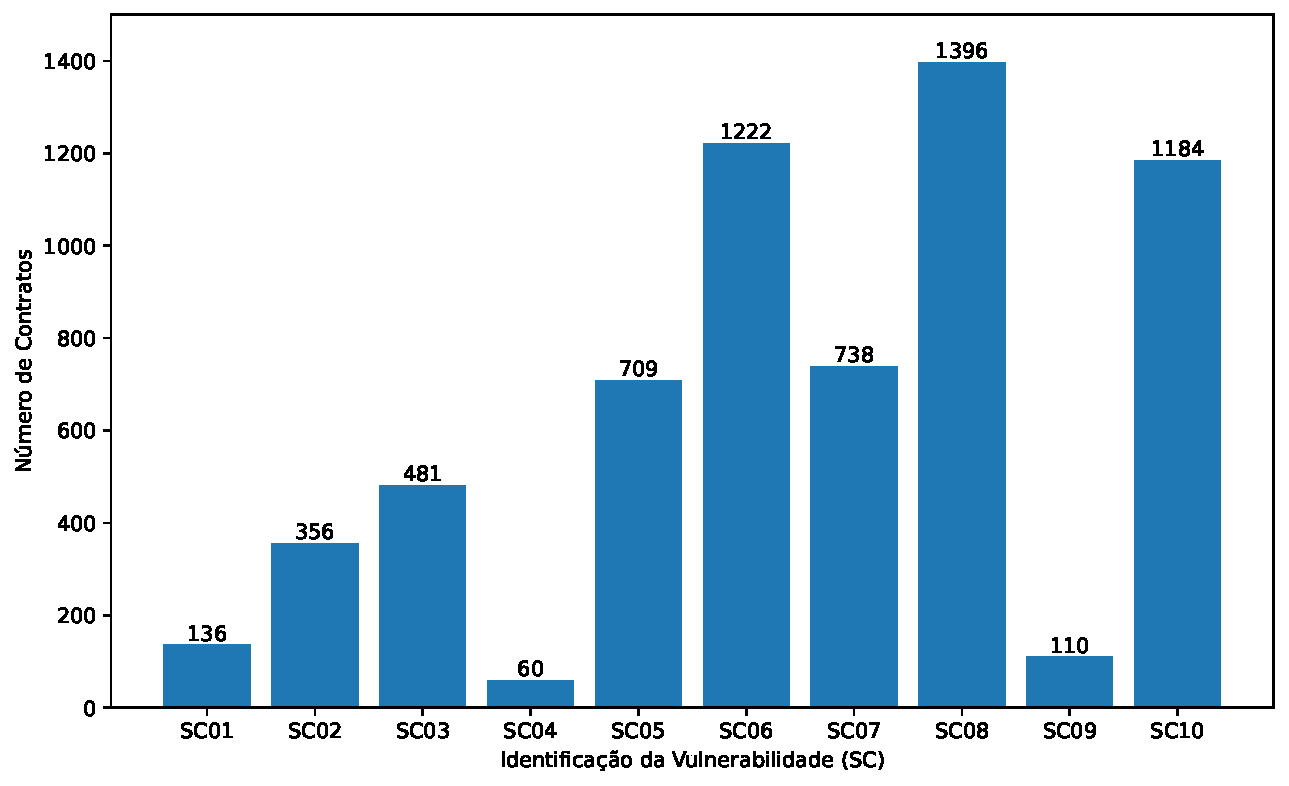
\includegraphics[width=0.75\linewidth]{images/grafico_dataset.pdf}
    \caption{Quantidade de contratos inteligentes por vulnerabilidade.}
    \label{fig:grafico_dataset}
\end{figure}

\subsection{Ferramentas Selecionadas}\label{subsec:selectedtools}

Para a condução deste estudo comparativo das ferramentas de detecção de vulnerabilidades em contratos inteligentes na blockchain Ethereum, nós selecionamos três ferramentas representativas que empregam diferentes abordagens de análise: Slither, Mythril, ConFuzzius.
% A Tabela~\ref{tab:tools} resume as características de cada ferramenta.


% \begin{table}[!ht]
%     \centering
%     \caption{Ferramentas selecionadas para análise.}
%     \begin{tabular}{|c|c|}
%     \hline
%         \textbf{Ferramenta} & \textbf{Técnica principal} \\
%     \hline
%         Slither & Execução simbólica \\
%     \hline
%         Mythril & Verificação Formal \\
%     \hline
%         ConFuzzius & \textit{Fuzzing} \\
%     \hline
%     \end{tabular}
%     \label{tab:tools}
% \end{table}

Cada ferramenta foi selecionada por suas características particulares e abordagens distintas para análise de segurança. O Slither representa as ferramentas de análise estática baseadas em código-fonte \cite{feist2019slither}. Já o Mythril exemplifica técnicas de execução simbólica ao nível de \textit{bytecode} \cite{mythril2018}, e o ConFuzzius ilustra a abordagem híbrida com \textit{fuzzing} evolutivo \cite{9581164}. Esta diversidade metodológica permite uma comparação representativa do estado atual das principais técnicas de análise de segurança para contratos inteligentes. Além disso, apesar de em trabalhos anteriores como~\cite{kushwaha2022ethereum} serem apresentadas mais ferramentas disponíveis na literatura, nós constatamos que ferramentas como Oyente~\cite{luu2016making}, Vandal~\cite{brent2018vandal}, ContractFuzzer~\cite{jiang2018contractfuzzer}, foram descontinuadas e não recebem mais atualizações. Dessa maneira, comparamos as principais ferramentas que ainda recebem atualizações e lidam com as versões mais atuais da linguagem Solidity.

% Estas ferramentas foram executadas utilizando o conjunto de dados descrito na seção 4.1, o que possibilita uma avaliação equitativa de suas capacidades de detecção. Na sequência, apresentamos uma descrição de cada uma destas ferramentas, destacando suas principais características.

A ferramenta Slither converte o código Solidity em uma representação intermediária chamada SlithIR, que adota a forma \textit{Static Single Assignment} (SSA) e um conjunto reduzido de instruções, a fim de facilitar a implementação de análises mantendo a semântica do código \cite{feist2019slither}. A ferramenta emprega técnicas de análise de fluxo de dados e rastreamento de informações sensíveis (\textit{taint tracking}) para detectar vulnerabilidades que dizem respeito às funcionalidades implementadas de um contrato inteligente.

 % De acordo com \cite{feist2019slither}, o Slither "supera outras ferramentas de análise estática na detecção de problemas em contratos inteligentes da Ethereum em termos de velocidade, robustez e equilíbrio entre detecção e falsos positivos".

Já a ferramenta Mythril realiza análises através de três abordagens principais: execução simbólica, resolução SMT (\textit{Satisfiability Modulo Theories}) e análise de propagação de dados sensíveis (\textit{taint analysis}) \cite{kushwaha2022ethereum}. O módulo de execução simbólica LASER é responsável por simular o ambiente de execução dos contratos, permitindo que Mythril explore todos os estados possíveis de execução do contrato ao longo de múltiplas transações. A ferramenta utiliza também o teorema provador Z3, desenvolvido pela Microsoft Research, para validar ou refutar a existência de estados comprometidos \cite{sharma2022survey}.

O ConFuzzius apresenta uma estrutura composta por três componentes principais: o módulo de \textit{fuzzing} evolutivo, a Máquina Virtual Ethereum (EVM) com instrumentação e o componente de análise de traços de execução \cite{9581164}. O componente evolutivo da ferramenta utiliza um algoritmo genético para gerar sucessivas populações de casos de teste e intercala técnicas de \textit{fuzzing} com execução simbólica quando encontra ramificações complexas no código.

% \subsection{Configuração Experimental}\label{subsec:setup}

\section{Resultados}\label{sec:results}

Neste estudo analisamos as ferramentas Slither, Mythril e ConFuzzius para a detecção de vulnerabilidades em contratos inteligentes. A análise considerou os contratos específicos para cada vulnerabilidade listada na OWASP, conforme a Tabela \ref{tab:owasp_smart_contracts}. Nossos resultados indicam como cada ferramenta possui vantagens e desvantagens dependendo do caso de uso. A ConFuzzius apresenta-se como a ferramenta mais eficiente em tempo de execução, porém possui poucos (4) detectores de vulnerabilidades em relação às outras ferramentas. Por sua vez, a ferramenta Mythril apresenta detectores para todas (10) as vulnerabilidades estudadas, porém enfrenta desafios de escalabilidade para auditorias de vários contratos ao atingir tempos de execução altos em relação às outras ferramentas. Por fim, a ferramenta Slither apresenta tempos de execução próximos ao do ConFuzzius e cobre quase todas as vulnerabilidades estudadas (7), mostrando-se como uma ferramenta balanceada no quesito de escalabilidade \textit{versus} capacidade de detecção.

\subsection{Capacidade de Detecção}\label{subsec:detectionanalysis}

% As dez vulnerabilidades avaliadas estão organizadas da seguinte maneira: Access Control Vulnerabilities \textbf{(SC01)}, Price Oracle Manipulation \textbf{(SC02)}, Logic Errors \textbf{(SC03)}, Lack of Input Validation \textbf{(SC04)}, Reentrancy Attacks \textbf{(SC05)}, Unchecked External Calls \textbf{(SC06)} Flash Loan Attacks \textbf{(SC07)}, Integer Overflow and Underflow \textbf{(SC08)}, Insecure Randomness \textbf{(SC09)} e Denial of Service (DoS) Attacks \textbf{(SC10)}. 

Em relação a capacidade de detecção das vulnerabilidades do Top-10 do OWASP, é possível observar a acurácia das ferramentas na Figura~\ref{fig:analiseacuracia}. De acordo com o gráfico, as ferramentas Slither e Mythril possuem a capacidade de detectar uma maior variedade de vulnerabilidades dentre as ferramentas estudadas. Contudo, em casos como as vulnerabilidade SC06, SC08 e SC10 a ferramenta ConFuzzius possui uma acurácia maior.

\begin{figure}[!ht]
    \centering
    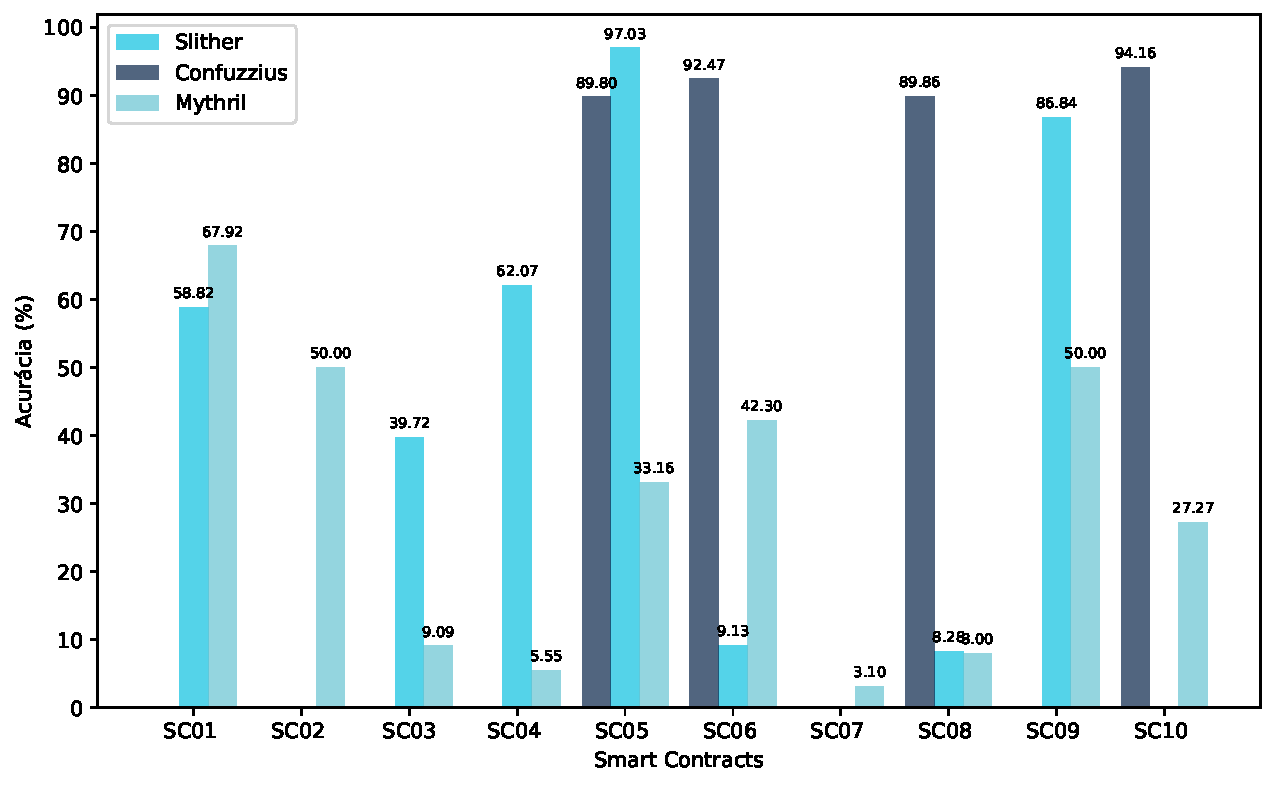
\includegraphics[width=0.75\textwidth]{images/grafico_acuracia.pdf} 
      \caption{Comparação de Acurácia das ferramentas Slither, ConFuzzius e Mythril.}
    \label{fig:analiseacuracia}
\end{figure}

A ferramenta ConFuzzius não possui detectores para todas as vulnerabilidades do Top-10, porém possui a melhor acurácia de detecção para as vulnerabilidades que a ferramenta consegue suportar. É possível observar também que, a vulnerabilidade SC07 possui a menor capacidade de detecção dentre as ferramentas analisadas. Uma justificativa para este resultado é que esta vulnerabilidade em particular não depende somente do código do contrato, mas também da ordem de execuções das transações que ocorrem na blockchain.

Dentre as três ferramentas, a ferramenta Mythril é a que possui um desempenho menor, que é justificado na Seção~\ref{subsec:performanceanalysis}. Para a maioria das vulnerabilidades a acurácia fica abaixo de 50\%. Porém, ela foi a única ferramenta que conseguiu detectar a vulnerabilidade SC02, que é uma vulnerabilidade que também depende do fluxo de execução do contrato na blockchain. A capacidade da Mythril detectar vulnerabilidades deste tipo baseia-se em seu método de combinar a execução simbólica com a instrumentação de instruções EVM.

Já a Figura \ref{fig:analisemetricas} apresenta o gráfico comparativo das três ferramentas em relação a quantidade de contratos analisados (CA), contratos verificados (CV), \textit{i.e.} contratos inteligentes analisados que foram encontradas vulnerabilidades, contratos em que a execução teve erros (E) e, por fim os contratos não-verificados (CNV), que são os contratos analisados, mas que as vulnerabilidades deles não foram identificadas pelas ferramentas. É possível observar que a métrica de erros (E) representa mais da metade de todo o conjunto de dados.

\begin{figure}[!ht]
    \centering
    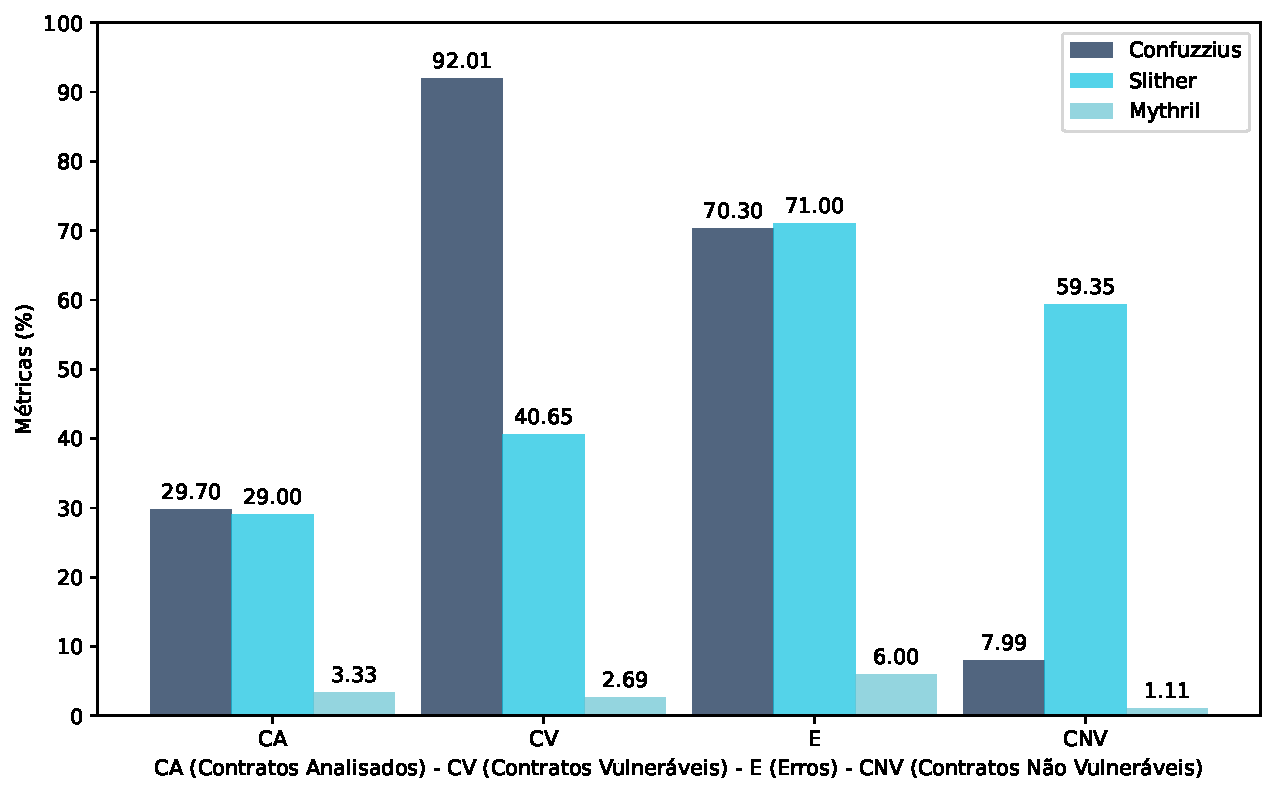
\includegraphics[width=0.75\textwidth]{images/grafico_metricas.pdf} 
      \caption{Análise de métricas das ferramentas Slither, ConFuzzius e Mythril.}
    \label{fig:analisemetricas}
\end{figure}

Durante as nossas medições, observamos que muitos contratos do conjunto de dados possuem versões da linguagem Solidity muito antigas, e as ferramentas acabam não suportando, pois uma das principais boas práticas de codificação de contratos é utilizar versões atuais da linguagem Solidity. Versões atuais da linguagem podem mitigar certas vulnerabilidades pelo próprio compilador atualizado. Vale ressaltar que, como o conjunto de dados utilizado é uma consolidação de outros trabalhos da literatura, destacamos a criação de conjunto de dados de contratos inteligentes vulneráveis atuais como um desafio em aberto.

Entretanto, é possível observar pela métrica CV como o ConFuzzius apesar de detectar poucas vulnerabilidades do OWASP, possui a melhor taxa de detecção de contratos, mostrando a confiabilidade e robustez da ferramenta. Já o Slither, possui mais contratos não-verificados (CNV), porém mantém uma taxa melhor em CV em vista da Mythril, ou seja, a ferramenta Slither acaba sendo versátil em cobrir mais vulnerabilidades, fornecendo uma visão geral sobre o código de um contrato inteligente. A ferramenta Mythril não consegue executar todo o conjunto de dados em tempo hábil para gerar resultados, o que justifica as métricas serem inferiores para esta ferramenta.

% Para melhor compreensão dos resultados, serão apresentados três gráficos principais: Comparação de Tempo,Acurácia da Análise e Métricas Comparativas.Esses gráficos proporcionarão uma visão clara da eficácia e do desempenho das ferramentas analisadas, permitindo uma comparação objetiva entre elas.


% Comparação de Tempo: Um gráfico ilustrando o tempo médio (em segundos) necessário para a execução das ferramentas Slither e ConFuzzius em cada contrato analisado.

% \begin{figure}[!ht]
%     \centering
%     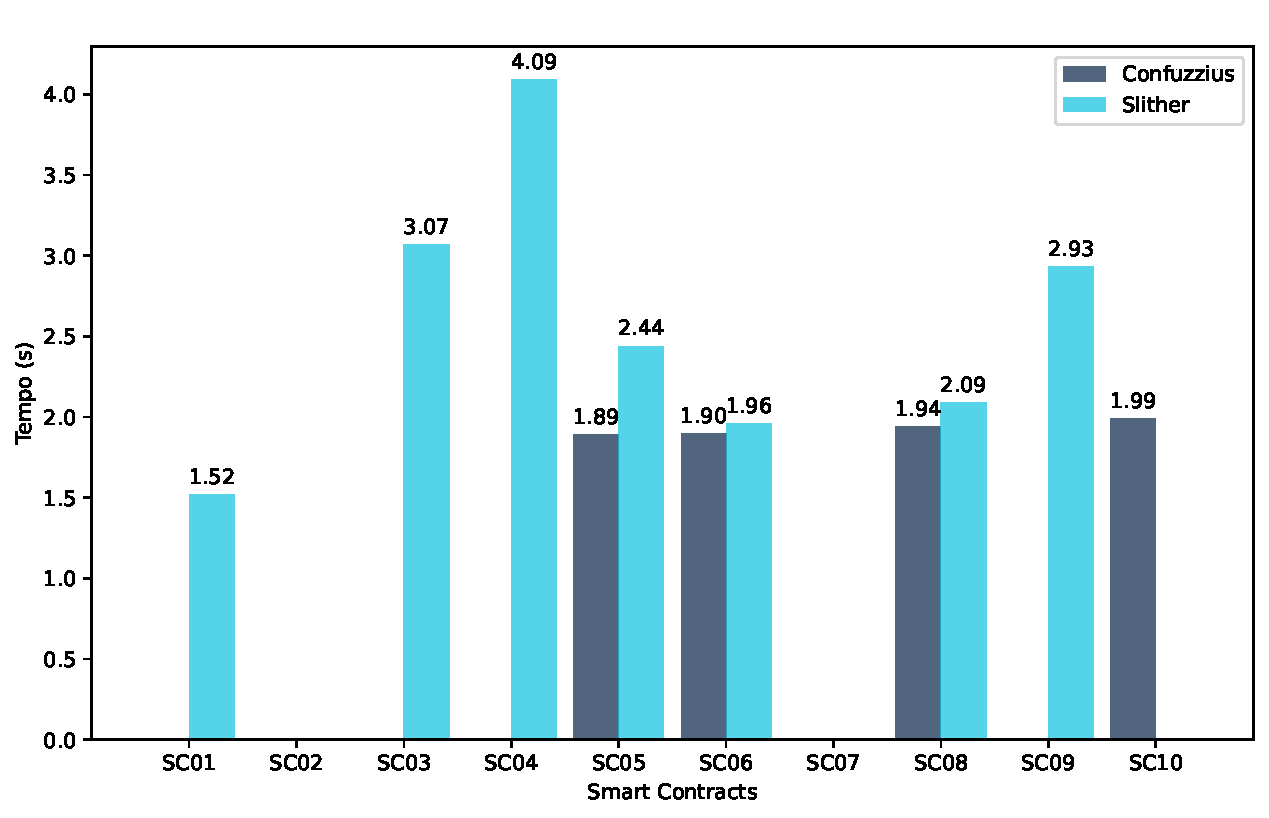
\includegraphics[width=1.0\textwidth]{images/grafico_tempo .pdf} 
%       \caption{Comparação de Tempo das ferramentas Slither e ConFuzzius}
%     \label{fig:analisetempo}
% \end{figure}
% Acurácia da Análise: Um gráfico demonstrando a porcentagem média de acurácia alcançada por Slither e ConFuzzius na análise de cada vulnerabilidade.


% Métricas Comparativas: Um gráfico contendo os seguintes parâmetros de desempenho das ferramentas Slither e ConFuzzius: \textbf{(CA)} Número de contratos analisados com sucesso,\textbf{(CV)}Número de contratos nos quais a vulnerabilidade correspondente foi identificada,\textbf{(E)}Número de contratos que não puderam ser analisados devido a incompatibilidade de versão ou erros sintáticos,\textbf{(CNV)} Número de contratos analisados, mas nos quais nenhuma vulnerabilidade foi detectada.




%A \textbf{Tabela 2 - Métricas de Desempenho da ferramenta ConFuzzius} apresenta os resultados obtidos executando a ferramenta \textbf{ConFuzzius}. \begin{table}[!ht]
  %  \centering
   % \label{tab:analise-ferramenta-confuzzius}
    %\resizebox{\textwidth}{!}{%
   % \begin{tabular}{|c|c|c|c|c|c|c|c|c|}
     %   \hline
     %   \multicolumn{8}{|c|}{\textbf{ConFuzzius}} \\ \hline
      %  \textbf{SC} & \textbf{Tempo(s)} & \textbf{Cobertura (\%)} & \textbf{DataSet} & \textbf{CA} & \textbf{CV} & \textbf{E} & \textbf{CNV} \\ 
     %   \hline
      %  SC01 & -  & -  & 136  & -  & -  & -  & -  \\ \hline
      %  SC02 & -  & -  & 356  & -  & -  & -  & -  \\ \hline
      %  SC03 & -  & -  & 481  & -  & -  & -  & -  \\ \hline
       % SC04 & -  & -  & 60   & -  & -  & -  & -  \\ \hline
       % SC05 & 1.89  & 89.80\%  & 709  & 196  & 176  & 513  & 20  \\ \hline
       % SC06 & 1.9  & 92.47\%  & 1222  & 292  & 270  & 930  & 22  \\ \hline
        %SC07 & -  & -  & 738  & -  & -  & -  & -  \\ \hline
       % SC08 & 1.94  & 89.86\%  & 1396  & 355  & 319  & 1041  & 36  \\ \hline
       % SC09 & -  & -  & 110  & -  & -  & -  & -  \\ \hline
       % SC10 & 1.99  & 94.16\%  & 1184  & 497  & 468  & 687  & 29  \\ \hline
   % \end{tabular}%
   % }
   % \caption{Métricas de desempenho da ferramenta ConFuzzius}
%\end{table}

%A \textbf{Tabela 3 - Métricas de Desempenho da ferramenta Slither} apresenta os resultados obtidos executando a ferramenta \textbf{Slither}. 
%\begin{table}[!ht]
  %  \centering
 %   \label{tab:analise-ferramenta-slither}
   % \resizebox{\textwidth}{!}{%
   % \begin{tabular}{|c|c|c|c|c|c|c|c|c|}
    %    \hline
    %    \multicolumn{8}{|c|}{\textbf{Slither}} \\ \hline
     %   \textbf{SC} & \textbf{Tempo(s)} & \textbf{Cobertura (\%)} & \textbf{DataSet} & \textbf{CA} & \textbf{CV} & \textbf{E} & \textbf{CNV} \\ 
      %  \hline
      %  SC01 & 1.52  & 58,82\%  & 136  & 51  & 30  & 85  & 21  \\ \hline
     %  SC02 & -  & -  & 356  & -  & -  & -  & -  \\ \hline
        %SC03 & 3.07  & 39.72\%  & 481  & 214  & 85  & 267  & 129  \\ \hline
       % SC04 & 4.09  & 62.07\%  & 60   & 29  & 18  & 31  & 11  \\ \hline
        %SC05 & 2.44  & 97.03\%  & 709  & 202  & 196  & 507  & 6  \\ \hline
       % SC06 & 1.96  & 19.13\%  & 1222  & 298  & 57  & 924  & 241  \\ \hline
        %SC07 & -  & -  & 738  & -  & -  & -  & -  \\ \hline
        %SC08 & 2.09  & 18.28\%  & 1396  & 361  & 66  & 1035  & 295  \\ \hline
       % SC09 & 2.93  & 86.84\%  & 110  & 38  & 33  & 72  & 5  \\ \hline
       % SC10 & -  & -  & 1184  & -  & -  & -  & -  \\ \hline
   % \end{tabular}%
  %  }
   % \caption{Métricas de desempenho da ferramenta Slither}
%\end{table}
%\begin{table}[!ht]
   % \centering
    %\label{tab:analise-ferramenta-Mythril}
   % \resizebox{\textwidth}{!}{%
  %  \begin{tabular}{|c|c|c|c|c|c|c|c|c|}
     %   \hline
      %  \multicolumn{8}{|c|}{\textbf{Mythril}} \\ \hline
      %  \textbf{SC} & \textbf{Tempo(h)} & \textbf{Cobertura (\%)} & \textbf{DataSet} & \textbf{CA} & \textbf{CV} & \textbf{E} & \textbf{CNV} \\ 
      %  \hline
      %  SC01 &  34.49 & 67,92\%  & 136  & 53  & 36  & 26  & 17  \\ \hline
     %   SC02 &  5.52 & 50,00\%  & 356  & 10  & 7  & 4  & 3  \\ \hline
      %  SC03 &  7.45 & 9,09\%  & 481  & 4  & 1  & 7  & 3  \\ \hline
       % SC04 & 5.35  & 5,55\%  & 60   & 7  & 5  & 2  & 2  \\ \hline
      %  SC05 & 40.48  & 33,16\%  & 709  & 100  & 65  & 96  & 35  \\ \hline
       % SC06 & 7.58  & 42,30\%  & 1222  & 12  & 11  & 14  & 1  \\ \hline
       % SC07 & 3.39  & 3,10\%  & 738  & 9  & 6  & 184  & 3  \\ \hline
       % SC08 & 9.18  & 8,00\%  & 1396  & 8  & 4  & 42  & 4  \\ \hline
        %SC09 & 8.24  & 50,00\%  & 110  & 5  & 4  & 3  & 1  \\ \hline
      %  SC10 & 8.33  & 27,27\%  & 1184  & 5  & 3  & 6  & 2  \\ \hline
   % \end{tabular}%
  %  }
  %  \caption{Métricas de desempenho da ferramenta Mythril}
%\end{table}

\subsection{Análise de Desempenho}\label{subsec:performanceanalysis}

A análise de desempenho das ferramentas ConFuzzius, Slither e Mythril revelou diferenças significativas tanto na cobertura de vulnerabilidades quanto na eficiência em tempo de execução, conforme a Tabela~\ref{tab:analise-tempo}. A ferramenta ConFuzzius demonstrou uma abordagem mais limitada em relação às vulnerabilidades detectadas, cobrindo apenas quatro das dez listadas no Top-10 da OWASP. No entanto, quando consegue identificar vulnerabilidades, apresenta uma acurácia alta, chegando a 89\%, com um tempo médio de execução inferior a 2 segundos por contrato. Esse desempenho é reforçado pelos resultados obtidos ao executar a ferramenta no conjunto de dados analisado: dos 4.511 contratos testados, 29,7\% foram analisados com sucesso e, desses, 92,01\% continham vulnerabilidades detectadas pela ferramenta. Apenas 7,99\% das vulnerabilidades passaram despercebidas. Entretanto, um grande percentual dos contratos (70,3\%) não foi testado, devido à erros de versão da linguagem Solidity.

Por outro lado, a ferramenta Slither se mostrou mais abrangente, detectando sete das dez vulnerabilidades do Top-10 da OWASP. Apesar dessa vantagem, seu desempenho em termos de acurácia foi inferior. A acurácia ficou em 18,28\%, e o tempo médio de execução foi inferior a 4 segundos por contrato, ou seja, mais lento que a ferramenta ConFuzzius. A Slither conseguiu analisar 4.114 contratos, dos quais 29\% foram analisados com sucesso. No entanto, a taxa de identificação de vulnerabilidades foi bem menor: apenas 40,65\% dos contratos testados apresentaram vulnerabilidades detectadas, enquanto 59,35\% passaram despercebidas. Assim como no ConFuzzius, um grande número de contratos (71\%) não foi testado por problemas similares de versão da linguagem.

% \begin{table}[!ht]
%    \centering
%    \label{tab:analise-tempo}
%     \resizebox{\textwidth}{!}{%
%    \begin{tabular}{|c|c|c|c|c|c|c|c|c|}
%        \hline
%        \multicolumn{8}{|c|}{\textbf{ConFuzzius}} \\ \hline
%        \textbf{SC} & \textbf{Tempo(s)} & \textbf{Cobertura (\%)} & \textbf{DataSet} & \textbf{CA} & \textbf{CV} & \textbf{E} & \textbf{CNV} \\ 
%        \hline
%        SC01 & -  & -  & 136  & -  & -  & -  & -  \\ \hline
%        SC02 & -  & -  & 356  & -  & -  & -  & -  \\ \hline
%        SC03 & -  & -  & 481  & -  & -  & -  & -  \\ \hline
%        SC04 & -  & -  & 60   & -  & -  & -  & -  \\ \hline
%        SC05 & 1.89  & 89.80\%  & 709  & 196  & 176  & 513  & 20  \\ \hline
%        SC06 & 1.9  & 92.47\%  & 1222  & 292  & 270  & 930  & 22  \\ \hline
%         SC07 & -  & -  & 738  & -  & -  & -  & -  \\ \hline
%        SC08 & 1.94  & 89.86\%  & 1396  & 355  & 319  & 1041  & 36  \\ \hline
%        SC09 & -  & -  & 110  & -  & -  & -  & -  \\ \hline
%        SC10 & 1.99  & 94.16\%  & 1184  & 497  & 468  & 687  & 29  \\ \hline
%    \end{tabular}%
%    }
%    \caption{Métricas de desempenho da ferramenta ConFuzzius}
% \end{table}

\begin{table}[!ht]
    \caption{Tempo de execução das ferramentas por vulnerabilidades.}
    \centering
    \begin{tabular}{|c|c|c|c|}
        \hline
        \textbf{SC} & \textbf{ConFuzzius} & \textbf{Slither} & \textbf{Mythril} \\
        \hline
        SC01 & - & 1,52s & 34,49h \\
        \hline
        SC02 & - & - & 5,52h \\
        \hline
        SC03 & - & 3,07s & 7,45h \\
        \hline
        SC04 & - & 4,09s & 5,35h \\
        \hline
        SC05 & 1,89s & 2,44s & 40,48h \\
        \hline
        SC06 & 1,9s & 1,96s & 7,58h \\
        \hline
        SC07 & - & - & 3,39h \\
        \hline
        SC08 & 1,94s & 2,09s & 9,18h \\
        \hline
        SC09 & - & 2,93s & 8,24h \\
        \hline
        SC10 & 1,99s & - & 8,33h \\
        \hline
    \end{tabular}
    \label{tab:analise-tempo}
\end{table}

Os resultados mostram que, enquanto Slither cobre mais tipos de vulnerabilidades, sua eficácia na detecção é menor. Por outro lado, ConFuzzius se sai melhor na identificação das vulnerabilidades que de fato cobre, com uma taxa de sucesso muito mais alta. No entanto, sua aplicação é mais limitada, pois consegue testar menos tipos de vulnerabilidades. Já a ferramenta Mythril, os resultados indicam que a ferramenta possui detectores para todas as dez vulnerabilidades listadas no Top 10 da OWASP. No entanto, seu desempenho variou significativamente entre as diferentes categorias de vulnerabilidades, com tempos de execução extremamente altos e baixa acurácia de detecção. A ferramenta apresentou uma cobertura média de apenas 12,79\% em relação ao conjunto de dados utilizado, com tempos de execução que variaram de 3,39 horas (SC07) a 40,48 horas (SC05). Em algumas vulnerabilidades, como SC01 (38,97\% de cobertura) e SC05 (27,64\%), a Mythril demonstrou eficiência moderada, enquanto em outras, como SC10 (0,92\%) e SC03 (2,28\%), sua detecção foi limitada.

Os resultados indicam que, em média, apenas 12,79\% dos contratos foram analisados com sucesso para a ferramenta Mythril. Dentre esses, a taxa de contratos vulneráveis detectados variou amplamente. Para os contratos que não foram testados, alguns dos fatores que interferiram nessas medições incluem: Erros devido às versões antigas da linguagem Solidity e o tempo alto para análise do contrato. Em uma análise de segurança, a Mythril demonstra que apesar de possuir uma variedade de detectores, não consegue finalizar a verificação de um contrato em tempo hábil, dificultando a usabilidade da ferramenta.

% Tendo isso em vista, pode-se concluir que a Mythril é uma ferramenta de analise bem concreta e funcional para diversos casos de vulnerabilidades em contratos inteligentes. Entretanto apresenta um desempenho muito complexo e demorado, podendo afetar resultados em pesquisas em larga escala, onde é necessario analisar uma gama maior de dados de contratos.
\section{Considerações Finais}\label{sec:conclusion}

Este trabalho apresenta um estudo comparativo as ferramentas ConFuzzius, Slither e Mythril para a detecção automática de vulnerabilidades em contratos inteligentes. Nas análises realizadas, foi utilizado um conjunto de dados com contratos inteligentes auditados manualmente por pesquisadores e especialistas, considerando as vulnerabilidades mais comuns de acordo com a OWASP para o ano de 2025.

A ferramenta ConFuzzius teve um tempo médio inferior a 2 segundos por vulnerabilidade e, apesar de testar apenas uma fração pequena do conjunto de dados, obteve alta taxa de detecção (92,01\%). Por outro lado, a ferramenta Slither testou uma quantidade maior de contratos, dos quais 29\% foram analisados com sucesso, porém sua taxa de identificação de vulnerabilidades foi de apenas 40,65\%, mantendo um tempo de execução semelhante. Já a ferramenta Mythril, embora ofereça detectores para todas as vulnerabilidades listadas, apresentou uma cobertura média de apenas 12,79\% do conjunto de dados devido aos tempos de execução que aumentaram significativamente em comparação as outras duas (podendo chegar até 40,48 horas ao analisar determinada vulnerabilidade) e variações de cobertura que vão de 0,92\% a 38,97\%.

Para análises que exigem maior precisão dentro de um escopo limitado, o ConFuzzius se mostra mais confiável e robusto, enquanto o Slither pode ser utilizado para uma abordagem mais abrangente, apesar de sua menor eficácia. Para análises em larga escala, a ferramenta Mythril demonstra como sendo inutilizável pelo fato de não conseguir retornar resultados em tempos satisfatórios, porém possui versatilidade em identificar vulnerabilidades que saem do escopo do código do contrato. Desafios comuns, como erros de versão e incompatibilidades, apontam para a necessidade de conjunto de dados com contratos inteligentes vulneráveis mais atuais, assim como há a necessidade por ferramentas de código-aberto com diferentes técnicas e que sejam mantidas continuamente. De modo geral, os resultados evidenciam que cada ferramenta apresenta vantagens e limitações, exigindo pesquisas e a resolução destes desafios em aberto na área de análise automática de contratos inteligentes. Como direções futuras, elencamos a criação de novas ferramentas que combinam diferentes técnicas e vantagens das ferramentas analisadas, assim como a definição de conjuntos de dados que representam o contexto atual da linguagem de codificação de contratos inteligentes.

\section{Agradecimentos}\label{sec:acknowledgements}
O presente trabalho foi realizado com o apoio do projeto ILIADA - A nova Internet da confiança, financiado pelo MCTI com recursos oriundos da Lei das TICs -Lei nº 8.248, de 23 de outubro de 1991, no âmbito do PPI-SOFTEX, coordenado pela Softex e publicado PDI 03, DOU 01245.023862/2022-14. Gostaríamos também de agradecer o apoio financeiro da CAPES, Fapemig e CNPq.

\bibliographystyle{sbc}

\bibliography{sbc-template}

\end{document}
